\section{Situation \& Problems}
%situation:
{\setbeamertemplate{frame footer}{\href{https://en.wikipedia.org/wiki/Dahuofang_Water_Tunnel}{\textcolor{gray}{\tiny{*https://en.wikipedia.org/wiki/Dahuofang\_Water\_Tunnel}}}}
\begin{frame}[t]{Current situation}
\begin{columns}[T]
\column{0.55\textwidth}
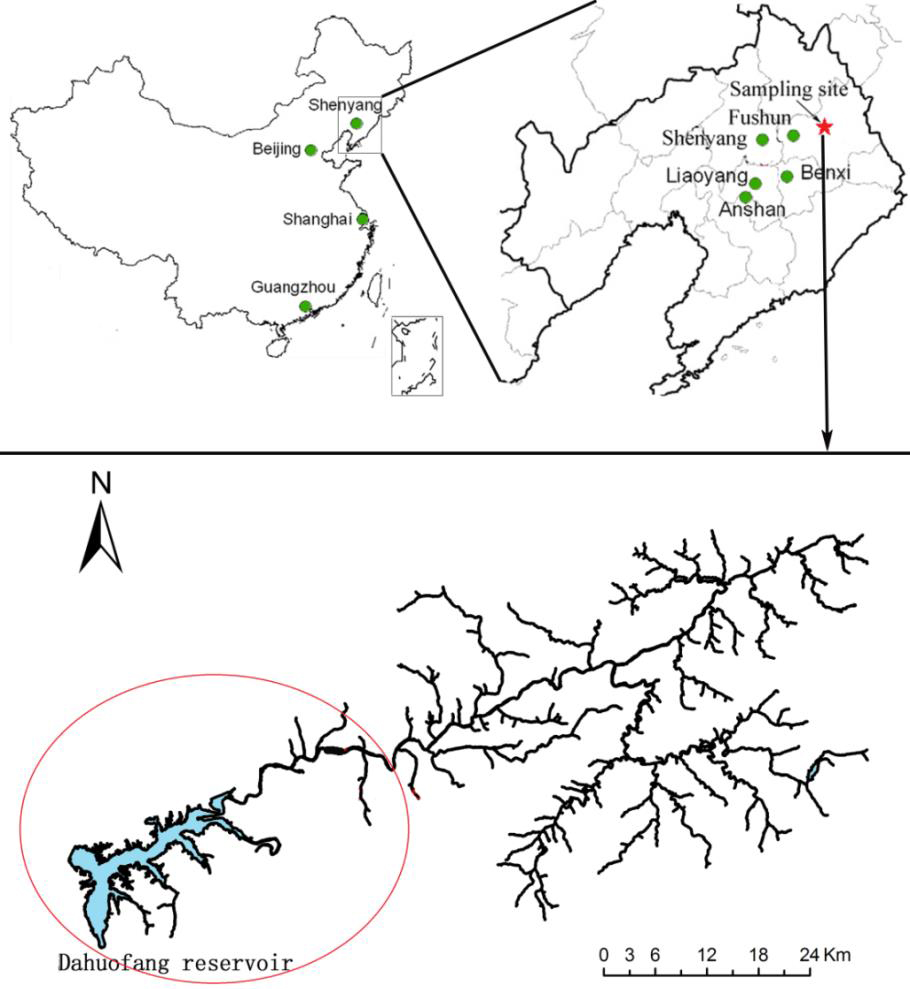
\includegraphics[height=0.8\textheight]{study_area.jpg}
\column{0.45\textwidth}
	\begin{itemize}
		\item Built in 1954--1958,\\first reservoir ``Made in\\ P.\ R.\ China''\\(not first one in China)
		\item Water source of city group in the lower reaches		
		\item Surface: 110 $km^2$,\\ 7 bil.\ $m^3$ water for\\ \alert{12 mil.} people per year
		\item Dahuofang Water Tunnel,\\built in 2006--2009,\\85.3 km long,\\8 m in diameter,\\\alert{cost: \$750 mil.}*
	\end{itemize}
\end{columns}
 \end{frame}
}

%problems:
\begin{frame}[t]{Main problems}
	\begin{itemize}[<+- | alert@+>]
		\item Water pollutants: NH$_3$-N (9.73 mg/L, 3.87 times higher) and TP (0.84 mg/L, 1.1 times higher)
		\item River bank damaged, riparian vegetation destroyed
		\item Wetland degraded, soil and water conservation capacity decreased
		\item Water-conservation-stands (WCS) structure single and simple, ecological functions lost
	\end{itemize}

\begin{columns}[T]
	\column{0.33\textwidth}
	\uncover<2->{\alert<2>{\frame{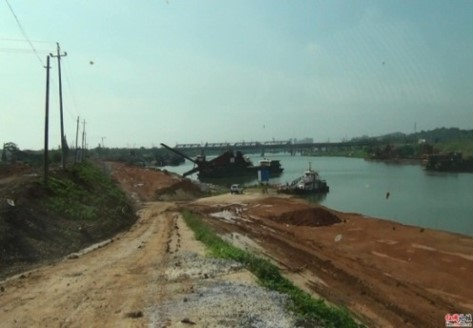
\includegraphics[width=\textwidth]{river_bank_damaged.jpg}}}}
		
	\column{0.33\textwidth}
	\uncover<3->{\alert<3>{\frame{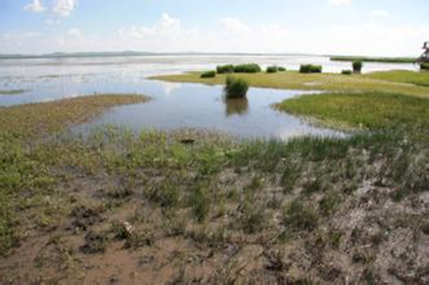
\includegraphics[width=\textwidth]{wetland_degraded.png}}}}	
	
	\column{0.33\textwidth}
	\uncover<4->{\alert<4>{\frame{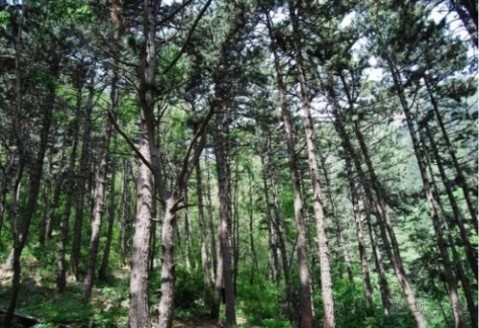
\includegraphics[width=\textwidth]{water_conservation_stands_structure_single.jpg}}}}
\end{columns}
\end{frame}